\documentclass[letterpaper]{article}
\usepackage{amssymb}
\usepackage{amsfonts}
\usepackage{amsmath}
\usepackage{stmaryrd}
\usepackage{graphicx}
\usepackage{subfigure}
\usepackage{pslatex}   % Good fonts psType 1 or \usepackage{mathptmx}
\usepackage{varioref}  % smart page, figure, table, and equation referencing
\usepackage{algorithm}
\usepackage{algorithmic}
%\usepackage{algorithm2e}
\usepackage{cancel}
\usepackage[small]{caption}
\usepackage{cancel}
\usepackage{tikz} 
\usepackage{pgf}
%\usepackage{fancy headings}

  \newcommand{\eqnref}[1]{Eq. (\ref{#1})}                % Eq. (no)
  \newcommand{\figref}[1]{Figure \ref{#1}}                % Figure (no)
  \newcommand{\tblref}[1]{Table \ref{#1}}                % Table (no)
  \newcommand{\secref}[1]{Section \ref{#1}}                % Section (no)
  \newcommand{\incfig}{\centering\includegraphics*}  % Centered 
  \newcommand{\comment}[1]{\COMMENT{ \textcolor{blue}{ #1} }  }

%DG integrals
\newcommand{\pd}[2]{\frac{ \partial #1}{\partial #2}}
\newcommand{\volint}[1]{ \sum_{e \in \mathcal{T}_{h}}\int_{\Omega_k} #1 d\Omega_{e} }  
\newcommand{\surfint}[1]{\sum_{i\in \mathcal{I}_{h}}\int_{\Gamma^{i}} #1 ds}
\newcommand{\bsurfint}[1]{\sum_{b\in \mathcal{B}_{h}}\int_{\Gamma^{b}} #1 ds}
% Operators
\newcommand{\frechd}[2]{ #1'_{\left[ #2 \right]} }%\left( #3\right)} 
\newcommand{\diver}[1]{\nabla \cdot #1}
\newcommand{\abs}[1]{\left \lvert #1 \right \rvert}
\newcommand{\avg}[1]{\left\{ #1 \right\} }
\newcommand{\jump}[1]{\llbracket #1 \rrbracket}
\newcommand{\mat}[1]{\left[ #1 \right]}
\newcommand{\paren}[1]{\left( #1 \right)}
\newcommand{\sparen}[1]{\left[ #1 \right]}
\newcommand{\twonorm}[1]{\parallel #1 \parallel_{2}}
%variables
\newcommand{\hb}[1]{ {\bf #1}_{h} } % \hb for discrete symbol _{h} and bolded for vector in fields
% Fluxes 
\newcommand{\fc}{\vec{{\bf F}}_{c} \paren{\hb{u}}   }
\newcommand{\fv}{\vec{{\bf F}}_{v} \paren{\hb{u},\nabla \hb{u}} }
\newcommand{\fav}{\vec{{\bf F}}_{ad} \paren{ \epsilon,\hb{u},\nabla \hb{u} } }
\newcommand{\ec}{\vec{{\bf E}}_{c} \paren{\hb{u}}   }
\newcommand{\ev}{\vec{{\bf E}}_{v} \paren{\hb{u},\nabla \hb{u}} }
\newcommand{\eav}{\vec{{\bf E}}_{ad} \paren{ \epsilon,\hb{u},\nabla \hb{u} } }

\newcommand{\hc}{\mathcal{H}_{c} \paren{ \hb{u}^{+},\hb{u}^{-},\vec{n} } }  
\newcommand{\hv}{\mathcal{H}_{v} \paren{ \hb{u},\hb{u}^{-},\phi_{i}^{+}, \phi_{i}^{-},\nabla \hb{u}^{+},\nabla \hb{u}^{-},
\vec{n} } }
\newcommand{\hav}{\mathcal{H}_{ad}\paren{ \epsilon^{+},\epsilon^{-},\hb{u}^{+},\hb{w}^{+}, \hb{w}^{-},\hb{u}^{-},\nabla \hb{u}^{+},\nabla \hb{u}^{-},\vec{n} } }
\newcommand{\hcb}{\mathcal{H}_{c}^{b} \paren{ \hb{u}^{b} \paren{ \hb{u}^{+} },\vec{n} } } 
\newcommand{\hvb}{\mathcal{H}_{v}^{b} \paren{ \hb{u}^{b} \paren{\hb{u}^{+}},\phi_{i}^{+},\nabla \hb{u}^{+},\vec{n} } }
\newcommand{\havb}{\mathcal{H}_{ad}^{b} \paren{ \epsilon^{+}, \hb{u}^{b}\paren{ \hb{u}^{+}},{\bf w}^{+}, \nabla \hb{u}^{+},\vec{n} } }
%Non-linear variables
\newcommand{\Resid}[1] {{\bf R}(#1)}
\newcommand{\Residp}[1] {{\bf R}_{p}(#1)}
%FIgures
\newcommand{\figwidth}{.48\textwidth}
\newcommand{\lfigwidth}{.68\textwidth} %small version .68, large version .75
%%% Footer
%\lfoot[\fancyplain{}{}]{Approved for public release \\ distribution unlimited.}
\newcommand{\createav}{CREATE\textsuperscript{TM}-AV }

\title{Mesh}
\author{Nicholas K. Burgess}
\begin{document}
\maketitle
\section{Introduction} 
For the purposes of this document a mesh denotes a collection of nodes and elements.
nodes define points in physical space and elements describe how these nodes are connected.
The FEM library only supports certain types elements i.e. 1-D lines, 2-D
triangles, 2-D quadrilaterals, 3-D tetrahedra, 3-D prisms, and 3-D Hexahedra. First we
describe how elements are defined and how they are combined to form unstructured
meshes. Then with the theory how meshes are defined in hand we will describe the
data structures used in the code to define them and how to access the data of the mesh
using the implemented class functions of UnstGrid.
Note that mesh generation is a topic unto itself and the goal of this section is to
describe how the numerical integration library interacts with a pre-existing mesh. A
pre-existing mesh is one where the nodal coordinates in the physical space (i.e. the
one in which we wish to solve the PDE’s) represented notionally by the coordinates
$(x,y,z)$ are known. Additionally a mesh must supply how these nodes are connected
into elements along with how the boundary faces of the domain are connected to the
nodes that lie on the domain boundary. A few conditions on the mesh are that is must
be completely fill the domain of interest W, mathematically this is
\begin{equation}
\Omega = \bigcup_{e} \Omega_{e}
\end{equation}  

\section{Element Types}
This section describes the types of elements that are supported by the solver library.  In general elements define how nodes in the mesh are connected to each other.  Elements are normally defineds in a know standard space defined by greek letters $\xi, \eta, \zeta$.  The positions of the nodes of the elements are known in this standard space and the physical locations of the nodes in $(x,y,z)$ spaces are determined by a mapping function $f_{m}: \real^{d}\rightarrow \real^{d} $ where $d$ is the number of physical dimensions of the domain.  In this work the mapping functions $f_{m}$ take on the form of polynomial interpolations, that are nodally exact at all nodes of the element.       
 
\subsection{1-D Bar}
In one spatial dimension only one type of element is available.  This element in known as the ``bar'' element.  The ``bar'' element (shown in \figref{fig:c3_line}) is constructed by taking two nodes of the mesh and connecting them by a line segment.  
\begin{figure}[h!]
\centering
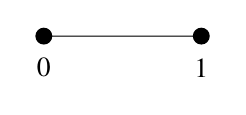
\begin{tikzpicture}
\draw[fill = black]  (0,0) circle (.1cm) -- (2,0) circle(.1cm) ;
\draw (0,-.4) node {0} (2,-.4) node {1};
\end{tikzpicture}
\caption{1-D ``bar'' element.}
\label{fig:c3_line}
\end{figure}

Recalling that each element has a definition in the standard space of equivalent dimension the coordinates of the nodes are node$_{1}$: $\xi = -1$ and node$_{2}$: $\xi = 1$ in the standard space spanning $\xi \in (-1,1)$.  

A 1-D ``bar'' element may have any number of solution unknowns associated with it but it requires a minimum of two uknowns: one for each element of the element.  For finite-element methods this results in a linear data representation and an asymptotically second-order accurate solution.  

\subsection{2-D Triangle}
In two spatial dimensions the simplex element shape is the triangle.  The triangle is defined by connecting 3 of the mesh nodes as in \figref{fig:c3_triangle}.  
\begin{figure}
\centering
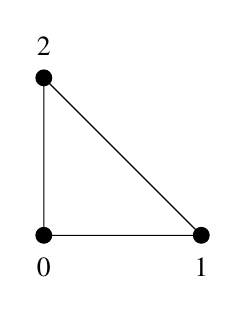
\begin{tikzpicture}
\draw[fill=black] (0,0) circle(.1cm) -- (2,0) circle(.1cm) -- (0,2) circle(.1cm) -- (0,0) circle(.1cm);
\draw (0,-.4)  node {0} (2,-.4) node {1} (0,2.4) node {2};
\end{tikzpicture}
\caption{2-D Triangle' element.}
\label{fig:c3_triangle}
\end{figure}
Triangles require a minimum of three nodes to define the element.  For a finite-element discretization these three nodes can be used to for a linear representation of the data within the element resulting in an asymptotically second order accurate approximation.   

\subsection{3-D Tetrahedron}
In three spatial dimensions the simplex element shape is the tetrahedron.  The tetrahedron is defined by a minimum of 4 nodes which are numbered 0 through 3.
\begin{figure}
\centering
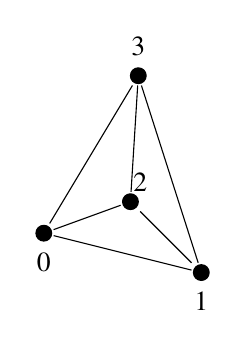
\begin{tikzpicture}[minimum size=1mm]
%\coordinate at (-1,0) circle(.1cm);
\node at (0,0) (Node1){};
\node at (2,-.5) (Node2) {};
\node at (1.1,.4) (Node3) {};
\node at (1.2,2) (Node4) {};
\draw[fill=black] (Node1) circle(.1cm);
\draw[fill=black] (Node2) circle(.1cm);
\draw[fill=black] (Node3) circle(.1cm);
\draw[fill=black] (Node4) circle(.1cm);
\draw (Node1) -- (Node2);
\draw (Node2) -- (Node3);
\draw (Node3) -- (Node4);
\draw (Node1) -- (Node3);
\draw (Node1) -- (Node4);
\draw (Node2) -- (Node4);
\node [black,below] at (Node1.south) {0};
\node [black,below] at (Node2.south) {1};
\node [black,above] at (Node3.east) {2};
\node [black,above] at (Node4.north) {3};
\end{tikzpicture}
\caption{3-D Tetrahadron.}
\label{fig:c3_tet}
\end{figure}
These four nodes can be used for a linear representation of the data within an element.  


\section{Mesh Connectivity}
The mesh connectivity data is stored in a linked list structure to facilitate optimal memory footprint.  Each connectivity of the mesh is stored as a separate linked list.  For example the nodes belonging to an element is one mesh connectivity and is stored in one linked list while the elements surrounding a node is stored in yet another linked list.  Each linked list is comprised of two arrays an ``index'' array and a ``data'' array.  The index array is normally named with an ``i'' at the end of the variable name and is composed on integer. 

As an example consider the connectivity defining the node numbers of each element in a mesh.  To make the explanation concrete consider the simple mesh in \figref{fig:c3_sample_mesh}.  
\begin{figure}[h!]
\centering
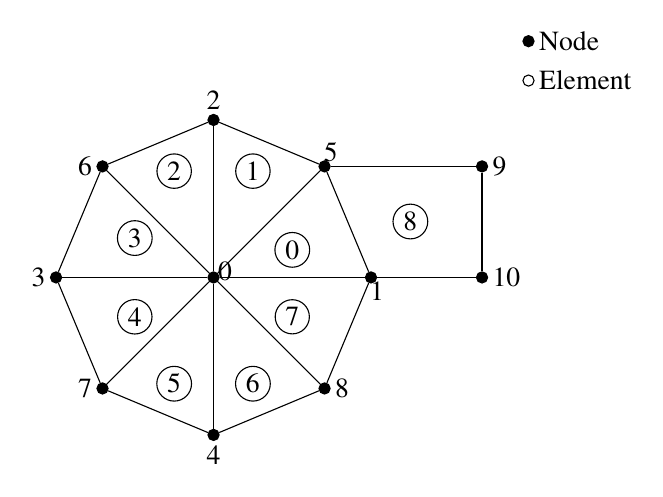
\begin{tikzpicture}[inner sep=.5mm,minimum size=.5mm]
\node at (0,0) [circle,draw=black,fill=black] (Node1) {};
\node at (2,0) [circle,draw=black,fill=black] (Node2) {};
\node at (0,2) [circle,draw=black,fill=black] (Node3) {};
\node at (-2,0) [circle,draw=black,fill=black] (Node4) {};
\node at (0,-2) [circle,draw=black,fill=black] (Node5) {};
\node at ( 1.41,1.41) [circle,draw=black,fill=black] (Node6) {};
\node at (-1.41,1.41) [circle,draw=black,fill=black] (Node7) {};
\node at (-1.41,-1.41) [circle,draw=black,fill=black] (Node8) {};
\node at (1.41,-1.41) [circle,draw=black,fill=black] (Node9) {};
\node at (3.41,1.41) [circle,draw=black,fill=black] (Node10) {};
\node at (3.41,0) [circle,draw=black,fill=black] (Node11) {};
\node [black,right] at (Node1.north) {0};
\node [black,below] at (Node2.east) {1};
\node [black,above] at (Node3.north) {2};
\node [black,left] at (Node4.west) {3};
\node [black,below] at (Node5.south) {4};
\node [black,above] at (Node6.east) {5};
\node [black,left] at (Node7.west) {6};
\node [black,left] at (Node8.west) {7};
\node [black,right] at (Node9.east) {8};
\node [black,right] at (Node10.east) {9};
\node [black,right] at (Node11.east) {10};
\draw (Node1) -- (Node2);
\draw (Node1) -- (Node3);
\draw (Node1) -- (Node4);
\draw (Node1) -- (Node5);
\draw (Node1) -- (Node6);
\draw (Node1) -- (Node7);
\draw (Node1) -- (Node8);
\draw (Node1) -- (Node9);
\draw (Node2) -- (Node6);
\draw (Node6) -- (Node3);
\draw (Node3) -- (Node7);
\draw (Node7) -- (Node4);
\draw (Node4) -- (Node8);
\draw (Node8) -- (Node5);
\draw (Node5) -- (Node9);
\draw (Node9) -- (Node2);
\draw (Node6) -- (Node10);
\draw (Node10) -- (Node11);
\draw (Node11) -- (Node2);
\node at (1,.35) [circle,draw=black] (elem1){0};
\node at (.5,1.35) [circle,draw=black] (elem2){1};
\node at (-.5,1.35) [circle,draw=black] (elem3){2};
\node at (-1,.5) [circle,draw=black] (elem4){3};
\node at (-1,-.5) [circle,draw=black] (elem5){4};
\node at (-.5,-1.35) [circle,draw=black] (elem6){5};
\node at (.5,-1.35) [circle,draw=black] (elem7){6};
\node at (1,-.5) [circle,draw=black] (elem8){7};
\node at (2.5,.71) [circle,draw=black] (elem9){8};
\node at (4,3) [circle,draw=black,fill=black] (nodelegend) {};
\node at (4,2.5) [circle,draw=black] (elemlegend) {};
\node  [black,right] at (nodelegend.east) {Node};
\node  [black,right] at (elemlegend.east) {Element} ;
\end{tikzpicture}
\caption{Sample Mesh.}
\label{fig:c3_sample_mesh}
\end{figure}
One should note that this 2-D example contains a mesh of mostly triangles with one quadrilateral.  The mixed element nature of the mesh prevents the mesh connectivity taking the form of a table (which can be stored in the computer a 2-D array) because some rows need more columns than others.  For example all rows of the table corrsponding to triangular elements require 3 columns and rows corresponding to quadrilaterals require 4 columns.  Clearly a more elegant data structure is required.  In this work a linked list is employed to facilitate the mesh connectivity storage.  
  
  Let \textit{element2node} denote the data array that stores the nodes that make up each element and \textit{element2nodei} denote the index array for \textit{elem2node}.  The size of \textit{element2node} is the sum of the nodes attached to each element over all elements of the mesh and the size of \textit{element2nodei} is the number of elements + 1.  For an element $e$ the nodes that makeup $e$ are stored in the following locations 
\begin{equation}
\begin{split}
 &  is = elem2nodei[e] \\
 &  ie = elem2nodei[e+1]-1 \\
 &  elem2node[is:ie]:\text{is where the nodes for element $e$ are stored}
\end{split}
\end{equation}

In order to make this concrete consider the sample mesh in \figref{fig:c3_sample_mesh}.  For this mesh the arrays \textit{element2nodei} and \textit{element2node} take the following values:
\begin{figure}
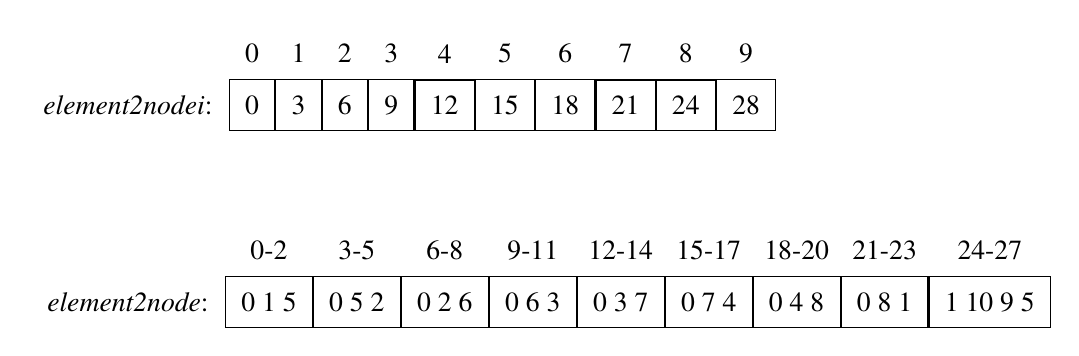
\begin{tikzpicture}[inner sep=2mm,minimum size = 2mm]
%Name
\node at(0,0) (namei) {\textit{element2nodei}:} ;
%Data 
\node at (namei.east)[rectangle,draw=black,right] (e0) {0} ;
\node at (e0.east)[rectangle,draw=black,right] (e1) {3} ;
\node at (e1.east)[rectangle,draw=black,right] (e2) {6} ;
\node at (e2.east)[rectangle,draw=black,right] (e3) {9} ;
\node at (e3.east)[rectangle,draw=black,right] (e4) {12} ;
\node at (e4.east)[rectangle,draw=black,right] (e5) {15} ;
\node at (e5.east)[rectangle,draw=black,right] (e6) {18} ;
\node at (e6.east)[rectangle,draw=black,right] (e7) {21} ;
\node at (e7.east)[rectangle,draw=black,right] (e8) {24} ;
\node at (e8.east)[rectangle,draw=black,right] (e9) {28} ;
%Address 
\node at (e0.north)[black,above] (a0) {0} ;
\node at (e1.north)[black,above] (a1) {1} ;
\node at (e2.north)[black,above] (a2) {2} ;
\node at (e3.north)[black,above] (a3) {3} ;
\node at (e4.north)[black,above] (a4) {4} ;
\node at (e5.north)[black,above] (a5) {5} ;
\node at (e6.north)[black,above] (a6) {6} ;
\node at (e7.north)[black,above] (a7) {7} ;
\node at (e8.north)[black,above] (a8) {8} ;
\node at (e9.north)[black,above] (a9) {9} ;

%Name
\node at (0,-2.5) (name) {\textit{element2node}:} ;
%Data 
\node at (name.east)[rectangle,draw=black,right] (d0) {0 1 5} ;
\node at (d0.east)[rectangle,draw=black,right] (d1) { 0 5 2 } ;
\node at (d1.east)[rectangle,draw=black,right] (d2) { 0 2 6 } ;
\node at (d2.east)[rectangle,draw=black,right] (d3) { 0 6 3 } ;
\node at (d3.east)[rectangle,draw=black,right] (d4) { 0 3 7 } ;
\node at (d4.east)[rectangle,draw=black,right] (d5) { 0 7 4 } ;
\node at (d5.east)[rectangle,draw=black,right] (d6) { 0 4 8 } ;
\node at (d6.east)[rectangle,draw=black,right] (d7) { 0 8 1 } ;
\node at (d7.east)[rectangle,draw=black,right] (d8) { 1 10 9 5 } ;
%Address 
\node at (d0.north)[black,above] (da0) {0-2} ;
\node at (d1.north)[black,above] (da1) {3-5} ;
\node at (d2.north)[black,above] (da2) {6-8} ;
\node at (d3.north)[black,above] (da3) {9-11} ;
\node at (d4.north)[black,above] (da4) {12-14} ;
\node at (d5.north)[black,above] (da5) {15-17} ;
\node at (d6.north)[black,above] (da6) {18-20} ;
\node at (d7.north)[black,above] (da7) {21-23} ;
\node at (d8.north)[black,above] (da8) {24-27} ;
%\draw [->] (e0.south) -- (da0.north);
%\draw [->] (e1.south) -- (da0.north);
\end{tikzpicture} 
\end{figure}

\section{Auxiliary Connectivity}
Solving partial differential equations (PDEs) numerically requires additional data structures beyond the nodes that make up an element.  In general the edges and or faces of the mesh must be extracted.  Additionally, one may need to form a list of nodes neighboring nodes or elements neighboring elements.  In general these structures are not available from the mesh generator but must be extracted by an algorithm.  Many of these data structures are formed as part of the mesh initialization process.  


\section{UnstGrid}
UnstGrid is a c++ class implements the methods required to store and work with an unstructured mesh of arbitrary and mixed element types.  The class assumes that the nodal coordinates and the mapping of which nodes make up an element will be provided in some form.  The basic usage of UnstGrid is described in the following algorithm
\begin{algorithm}[!h]
\caption{:Using UnstGrid}
\label{algsupg}
\begin{algorithmic}
 \STATE \comment{  First instantiate an object of type UnstGrid called grid.  This will have integer data of type int and real number data of type double.}
\STATE $UnstGrid<int,double>$ grid(3) \comment{Note that the class constructor is called with the number 3 indicating a 3-D grid}
\REQUIRE nnode, nelement, nbc\textunderscore{}face, nbc\textunderscore{}id;
\FOR { i = 0; i < nnode; i++}
\STATE \comment {Get values of x, y, z from wherever they are, these could be in a file or in some other data structure}
\STATE grid.set\textunderscore{}node\textunderscore{}coord(i, 0, x);
\STATE grid.set\textunderscore{}node\textunderscore{}coord(i, 1, y);
\STATE grid.set\textunderscore{}node\textunderscore{}coord(i, 2, z);
\ENDFOR
\FOR { e= 0; e < nelement; e++}
\STATE \comment{Get the nodes on the element and put them into the mesh data structure}
\FOR{n = 0; n < nnode\textunderscore{}on\textunderscore{}element; n++}
\STATE \comment {Knowing the nodes on an element from your mesh source populate the grid like this}
\STATE grid.set\_node\_on\_element(e, n, node) \comment{ Where node is the node number you want to assign as the nth node of element e}
\ENDFOR
\ENDFOR
\FOR { f= 0; f < nbc\_face; f++}
\STATE \comment{ Get the nodes on the element and put them into the mesh data structure}
\FOR{n = 0; n < nnode\textunderscore{}on\textunderscore{}bc\_face; n++}
\STATE \comment{ Knowing the nodes on an element from your mesh source populate the grid like this}
\STATE grid.set\_node\_on\_bc\_face(f, n, node) \comment{Where node is the node number you want to assign as the nth node of boundary face f}
\ENDFOR
\ENDFOR
\STATE \comment{Now use the init connectivity function to form all connectivity}
\STATE grid.init\textunderscore{}connectivity(); \comment{ Grid is now prepared for use}
\STATE \comment{ Mesh is ready for use}
\end{algorithmic}
\end{algorithm}
  

%%%%%%%%%%%%%%%%%%%%%%%%%%%%
\end{document}